\documentclass{article}


\usepackage{amsmath}
\usepackage{amssymb}
\usepackage{graphicx}
\usepackage{color}
\usepackage{subfig}
\usepackage{float} % For [H] placement

\usepackage[ruled,vlined,linesnumbered]{algorithm2e}

\usepackage{booktabs}

\usepackage[bookmarks=true,ocgcolorlinks=true,plainpages=false, breaklinks=true, bookmarksopen=true, bookmarksnumbered=true]{hyperref}
%\hypersetup{bookmarks=false}  %hide the bookmarks bar
%\hypersetup{bookmarksopen=false}  % expand tree of bookmarks or just show first level
\hypersetup{linkcolor=blue, citecolor=magenta,urlcolor=blue} % electronic
\hypersetup{colorlinks=true}

\usepackage[T1]{fontenc}
\usepackage{palatino}

\allowdisplaybreaks

\renewcommand{\vec}[1]{\ensuremath{{\boldsymbol #1}}}
\newcommand{\mat}[1]{\ensuremath{\boldsymbol{#1}}}

\newcommand{\unit}[1]{\textcolor{magenta}{#1}}
\newcommand{\brian}[1]{\textcolor{blue}{#1}}

\title{Statistical performance analysis of data-driven mesoscopic models}
\date{\today}

\begin{document}
\maketitle

\section{Introduction}
\label{sec:introduction}

\brian{What the paper is about / contribution}
This paper introduces the Bayesian Cramer Rao lower bound (BCRLB) to the neuroscience community. The BCRLB is an engineering method for evaluating the feasibility of constructing stochastic computational models from measured data. The lower bound defines the best possible outcome of estimating system states in terms of the levels of certainty. Although the methods and models discussed in this paper can be found dispersed in the engineering and computational neuroscience literature, respectively, it is important to link the fields together in order to advance our knowledge in systems neuroscience. \unit{this sentence is true, but I worry it downplays the contribution of the paper. presumably we will have some new conclusions? or maybe not}

\brian{Introduce the importance of the models, forward}
Mesoscopic mathematical models of the brain are becoming increasingly popular as tools for generating hypotheses on the physical principals that govern neurodynamics. Mesoscopic models describe the pooled dynamics of neural populations, analogous to signals recorded from a local field potential. Typically the state variables of models at this scale are the average membrane potential or the average firing rates of the neurons across the population (ref - Beurle, Wilson Cowan, Lopez Da Silva - van Rotterdam). More sophisticated models that describe higher-order statistics of neural populations have also been developed (Sompolinsky ?french guys? Jonathan Touboul). Forward models of this kind have led to theory on the emergence of the brains rhythms (Liley), the mechanisms of anesthetic agents (Liley - Dutch guys), the brain's response to sensory stimuli (Jansen and Ritt), short-term memory formation (Coombes), visual hallucinations (Cowan Bressloff, Ermentrout) and epileptic seizures (Freestone, Robinson, Wendling, Grimbert?, Terry). 

\brian{Introduce the importance of the models, inverse}
More recently, advances in engineering and statistical inference methods along with computing resources have expanded the utility of the mesoscopic models as integral elements of frameworks to estimate system states that can not be directly measured using electrophysiology (Friston, Freestone, Schiff, Terry). An established framework to reliably estimate physical properties underlying brain dynamics has the potential to revolutionize how we observe, diagnose, treat and cure neurological disorders. For example, in epilepsy the dynamics of hidden system and parametric states are thought to be highly patient-specific and unknown (Freestone - Book Chapter). Thus, the ability to estimate these quantities will enable a greater understanding of individual pathologies, leading to more tailored therapies and better patient outcomes.  Furthermore, subject-specific models will enable the application of control theory to the neurosciences, which is typically limited to man-made systems (Schiff Book).

\brian{Models are qualitative - need to validate properly - need to estimate parameters to do this}
To date, a large body of work has attempted to demonstrate the validity of mesoscopic neural models by qualitatively reproducing measured data. For example, establishing a match between a generative model's spectral profile with an electrophysiological measurement has typically been used as validation. In reality, such a demonstration does little more for neuroscience than generate hypotheses that are currently difficult to test. Having said this, many beautiful mathematical results have emerged that capture our imagination, but do not \emph{prove} anything about brain function. The reason why this is the case is that the models have inherent uncertainty (unknown inputs) and parameters of these models are difficult (if not impossible) to measure. Therefore, parameters are often tuned to obtain the required output. In order to truly validate theory, useful predictions must be made. However, testing predictions against measured data has not been standard practice since the parameters of the models are expected to vary across individuals and across disease states, making the testing difficult. It is clear that a systematic framework for estimating system variables is required to truly validate mesoscopic neural theory.

A critical step in establishing robust model fitting techniques is understanding the performance and feasibility of estimation algorithms. This paper introduces engineering tools to the neuroscience community for formally accessing the feasibility of estimating system variables. We also postulate how these tools can be used to increase performance of estimation methods that are important for patient-specific modeling. \unit{how does the CRLB help increase algorithm performance? seems a bit of a stretch.} The methods introduced in this paper can also be used to improve experiments to maximize the information content of measurements. This paper does not deal with model selection. Once models have been fit to subjects, a final step in assessing validity will be to examine the predictive power within a subject.  \unit{would be good to have a reference on model selection here}

\brian{Layout}
The remainder of the paper is arranged as follows. Section~\ref{sec:background} provides a description of the equations for a neural mass model. A derivation of the Bayesian Cramer Rao lower bound is presented in Section~\ref{sec:Theory}, followed by a description of the recursion required for applications involving filtering methods for state estimation. Next we provide a series of simulations that show how the bound is effected by measurement noise, and the variance of prior information. This is followed by a demonstration of how models with different structures have varying bounds, indicating how well we can possibly estimate the system states. The final simulation provides a comparison between bounds when the parameters of the models are set to obtain seizures-like patterns and alpha rhythm-like patterns. In the discussion section we provide further intuition into how the Bayesian Cramer Rao lower bound can help lead to advances in our knowledge and the development of theory in unlocking the secrets of the brain.

% If model does not work then it is hard to say why. For example, the model itself could be too complicated or an estimation method could not be good enough. Is an approximate filter good enough etc etc.


% Influence on sampling rate and estimation?
% of this framework History of models and estimation attempts
% Usefulness of bound: benchmark algorithms, experimental design, insight about inherent uncertainty -- which do we address
% Not claiming anything about which model is the 'best', but simply what level of complexity is possible - how increasing complexity affects uncertainty.

\section{Background}
\label{sec:background}


\paragraph{Neural Mass Model}
\begin{figure}[ht]
  \begin{center}
    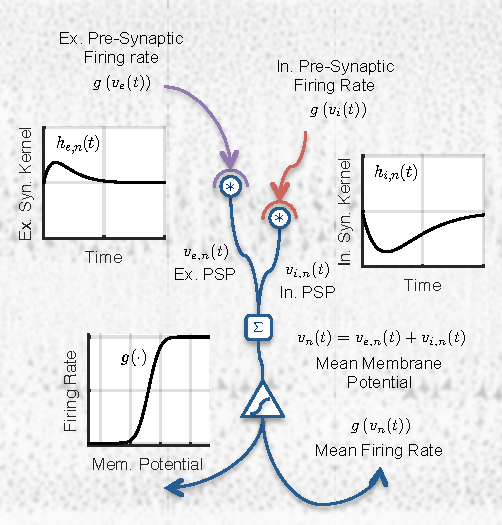
\includegraphics{./figures/pdf/SingleMass2.pdf}
  \end{center}
  \caption{\emph{\textbf{Neural Mass Model.} The soma of the neural mass is represented by the triangle and the synaptic connections are represented by the circles. The input mean firing rates, $g(v_{e}(t))$ and $g(v_{i}(t))$, are convolved with post-synaptic response kernels (PSRK), shown in the upper two insets, to give the excitatory and inhibitory post-synaptic membrane potentials (PSPs), $v_{e,n}(t)$ and $v_{i,n}(t)$, respectively. The PSPs are then summed and transformed by the sigmoid, shown in the lower inset, to give the output mean firing rate, $g(v_n(t))$. The neural mass may have any number of inputs and outputs. The firing rate on each of the outputs is equal.}}
  \label{fig:SingleNeuralMass}
\end{figure}
Neural mass models describe the mean firing rates and mean membrane potentials of populations of neurons. A graphical description of a single population neural mass model can be seen in Figure~\ref{fig:SingleNeuralMass}, showing the key elements including the post-synaptic response kernels and the sigmoidal activation function. 

To derive a standard neural mass model, we begin by defining the mean membrane potential of population $n$, $v_n(t)$, as the \brian{(average)} soma as the sum of all $M$ incoming mean post-synaptic membrane potentials
\begin{align}
	v_n(t) = \sum_m^M v_{m,n}(t).
\end{align}
Each of the post-synaptic membrane potentials results from a convolution between the input firing rate from population $m$, $g(v_m(t))$, with a post-synaptic response kernel, which is defined by
\begin{equation}\label{eq:conv_eq}
    v_{m,n}(t) = \frac{\alpha_{m,n}}{\tau_{m,n}}\int_{-\infty}^t  h_{m,n}(t-t')\phi_m(t') \,\mathrm{d}t'.
\end{equation}
The parameter $\alpha_{m,n}$ is the gain for the post-synaptic response kernel (PSRK), denoted by $h_{m,n}(t)$, from neural population $m$ to $n$, $\tau_{mn}$ is the membrane time constant, and $\phi(t)$ is the incoming mean firing rate. A common form of the PSRK is
\begin{equation}
    h_{mn}(t) = \eta(t)t\exp\left(-\frac{t}{\tau_{mn}}\right),
\end{equation}
where $\eta(t)$ is the Heaviside step function. An example of a PSRK can be seen in the left inset of Figure~\ref{fig:SingleNeuralMass}.  

The input firing rate to each population, $\phi_m(t)$, may come from a population that is explicitly modeled or an external input where
\begin{align}
	\phi_{m} =& \left\{ \begin{array}{lll} u_m  & \text{if } m \text{ indexes external inputs}\\
	g(v_m)  & \text{if } m \text{ indexes internal inputs} \end{array}\right. .
\end{align}
and $g(\cdot)$ is the sigmoidal activation function that relates the mean membrane potential the the mean firing rate of a population. The logistic function sigmoid is typically used and is described by 
\begin{align}
    g\left(v_n(t)\right) =& \frac{1}{1+\exp{\left(\varsigma_n\left(v_{0} - v_n(t)\right)\right)}}.
    \label{eq:sigmoid}
\end{align}
The quantity $\varsigma_n$ parametrizes the slope of the sigmoid (approximating the variance of firing thresholds within the populations) and $v_{0}$ describes the mean firing threshold relative to a mean rest potential. An example of the sigmoidal activation function can be seen in the lower inset of Figure~\ref{fig:SingleNeuralMass}.

The convolution in Equation~\ref{eq:conv_eq} can also be written as the ordinary differential equation (ODE)
\begin{equation}\label{eq:2ndOrder}
    \mathrm{D}v_n(t) = \frac{\mathrm{d}^2 v_n(t)}{\mathrm{d}t^2} + \frac{2}{\tau_{mn}}\frac{\mathrm{d} v_n(t)}{\mathrm{d}t} + \frac{1}{\tau_{mn}^2} v_n(t) = \frac{\alpha_{mn}}{\tau_{mn}} \phi_m(t),
\end{equation}
where $\mathrm{D}$ is a linear differential operator. To form a state-space model in a canonical format, Equation~\ref{eq:2ndOrder} is written as two coupled first-order ODEs by 
\begin{equation} \label{eq:2ndOrderNMM}
    \frac{\mathrm{d} v_n(t)}{\mathrm{d}t} = z_n(t),\,\,\,\,\,    \frac{\mathrm{d}z_n(t)}{\mathrm{d}t} = \frac{\alpha_{mn}}{\tau_{mn}} \phi_m(t) - \frac{2}{\tau_{mn}}z_n(t) - \frac{1}{\tau_{mn}^2} v_n(t).
\end{equation}

The parameters of the model, $\tau$, $\alpha$, $v_0$ and $\varsigma$, can be set so the neural mass has characteristics of a specific neural population, such as pyramidal neurons, spiny stellate cells and fast and slow inhibitory interneurons (GABA$_\mathrm{a}$ and GABA$_\mathrm{b}$). \unit{reference here} The neural masses can then be interconnected to represent the circuitry of a cortical column and further to form networks of columns. A small subset of the various kinds of neural mass models that have been explored \cite{Silva1974,Jansen1995,Wendling2002,David2003} are depicted in Figure~\ref{fig:NMMs}. Each synaptic connection in these networks can be described by the 2$^{\mathrm{nd}}$-order system of Equation~\ref{eq:2ndOrderNMM}, where the resultant dimensions (before simplification) of the networks of neural mass models in Figures~\ref{fig:NMMs} A, B, and C are 6, 12 and 18, respectively.
\begin{figure}[ht]
	\centering
		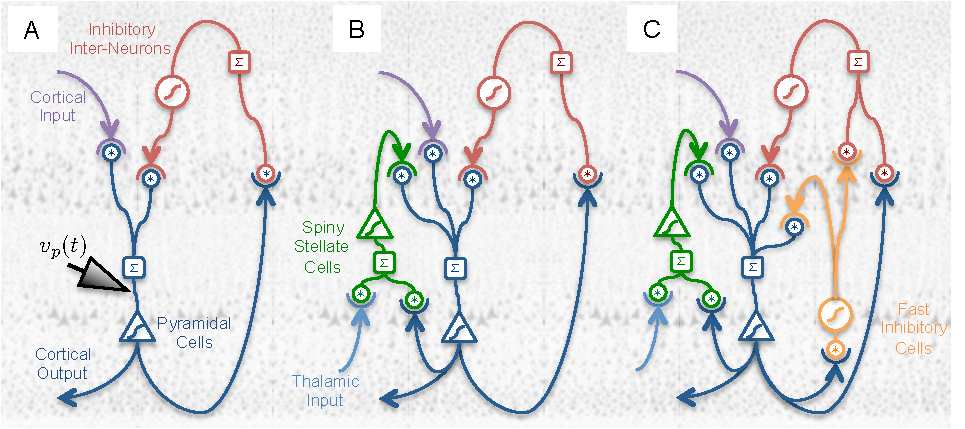
\includegraphics[scale=1]{./figures/pdf/NeuralMassesHoriz_plos2.pdf}
	\caption{\emph{\textbf{Models of Cortical Columns.} Each model has a pyramidal neural population, with various forms of feedback and inputs. Measurements from the model are derived from the mean membrane potential of the pyramidal population, $v_p(t)$, with additive noise.  a) Minimal model of a column with inhibitory feedback \cite{Silva1974}. b) An extension with excitatory feedback and afferent input from thalamus \cite{Jansen1995,David2003}. c) Column with inhibition occurring across two times scales, enabling modeling of higher frequency activity observed in seizures~\cite{Wendling2002}.}}
	\label{fig:NMMs}
\end{figure}

\begin{figure}[ht]
	\centering
		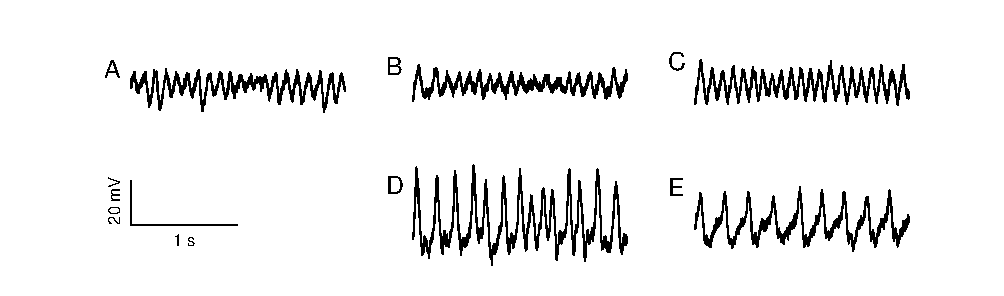
\includegraphics[scale=1]{./figures/pdf/Example_Data.pdf}
		\caption{\textbf{Example data generated using the neural mass models.}}
	\label{fig:NMMs}
\end{figure}

The higher dimensional models of cortical regions can be written in the form
\begin{align}
	\dot{\mathbf{x}} = \mathbf{A}\mathbf{x} + \mathbf{B} g\left(\mathbf{C}\mathbf{x}\right) + \mathbf{D}\mathbf{u},
\end{align}
where $\mathbf{x} \in \mathbb{R}^{N_x}$ is a state vector representing the postsynaptic membrane potentials generated by each population synapse and their time derivatives. There are two states per synapse and $N_x = 2N$ is the total number of states, where for $N$ synaptic connections in the models the state vector is of the form
\begin{align}
	\mathbf{x} = \begin{bmatrix} v_{1} & z_{1} & \hdots & v_{N} & z_{N}  \end{bmatrix}\unit{^\top}.
\end{align}
\unit{I wonder if x should have time dependence explicit, e.g., x(t) in 8 and 9}
The matrix $\mathbf{A}$ encodes the dynamics induced by the membrane times and for $N$ synapses has the block diagonal structure
\begin{align}
	\mathbf{A} = \mathrm{diag}\left(\begin{array}{ccc}\boldsymbol{\Psi}_1 & \hdots & \boldsymbol{\Psi}_N\end{array}\right),
\end{align}
where
\begin{align}
	\boldsymbol{\Psi}_n = \begin{bmatrix} 0 & 1 \\ -\frac{1}{\tau_n^2} & -\frac{2}{\tau_n} \end{bmatrix}.
\end{align}
The matrix of synaptic gains from internal inputs, $\mathbf{B}$, has the diagonal form 
\begin{align}
	\mathbf{B} = \mathrm{diag}\left(\begin{array}{cccccccc} 0 & \alpha_1 & \hdots & 0 & \alpha_{N-K} & \hdots & 0 & 0 \end{array}\right),
\end{align}
where $K$ is the number of external inputs. The synaptic gains of post-synaptic potentials that are generated from external inputs are captured by the input gain matrix $\mathbf{D}$. The adjacency matrix, $\mathbf{C}$, defines the connectivity structure of the model. It is a matrix of zeros or ones that defines all the connections between the cell population types (excluding external inputs) 
\begin{align}
	\mathbf{C} = \begin{bmatrix} 0 & 0 & \hdots & 0 & 0 \\
	\mathbf{c}_{2,1} & 0 &  & \mathbf{c}_{2,2(N-K)-1} & 0 \\ 
	\vdots & &  & & \vdots \\
	0 & 0 & \ddots & 0 & 0 \\
 	\mathbf{c}_{2(N-K),1} & 0 &  & \mathbf{c}_{2(N-K),2(N-K)-1} & 0 \\
	\vdots & & & & \vdots \\
	0 & 0 & & 0 & 0 \\
	0 & 0 & \hdots & 0 & 0 \end{bmatrix}. 
\end{align}
For example, if the PSPs from synapses 1 and 2 are summed and transformed by the sigmoid to give the input firing rate to synapse $n$, then row $2n$ of $\mathbf{C}$ with have the form
\begin{align}
	c_{2n,:} = \begin{bmatrix} 1 & 0 & 1 & 0 & 0 & 0 & \hdots & 0 & 0 \end{bmatrix}.
\end{align}
As mentioned above, $\mathbf{D}$ is a diagonal matrix of synaptic gains for connections from external sources where
\begin{align}
	\mathbf{D} = \mathrm{diag} \left(\begin{array}{cccccccc}0 & 0 & \hdots & 0 & \alpha_{N-K+1} & \hdots & 0 & \alpha_N\end{array}\right).
\end{align}

It is necessary to discretize the model to \unit{numerically} integrate the equations and run simulations. The discrete time version of the model is 
\begin{align}
	\dot{\mathbf{x}}_{t+\delta} = \mathbf{A}_{\delta}\mathbf{x}_t + \mathbf{B}_{\delta} g\left(\mathbf{C}\mathbf{x}_t\right) + \mathbf{D}_{\delta}\mathbf{u}_t,
\end{align}
\unit{what is $\dot x_{t+\delta}$? do you just mean $x_{t+\delta}$? or is the derivative a finite difference here?}
where $\delta$ is the integration time step. The matrices $\mathbf{A}_{\delta}$, $\mathbf{B}_{\delta}$ and $\mathbf{D}_{\delta}$ are discrete time versions of $\mathbf{A}$, $\mathbf{B}$ and $\mathbf{D}$, respectively, and are defined in Appendix~\ref{app:discretization}. For ease of notation, we shall abbreviate increments or decrements in time (by the integration time step) by $t+1$ or $t-1$, respectively. For the discrete time version of the model, the input $\mathbf{u}_t$ may be stochastic. A discrete time Gaussian input $\mathbf{u}_t\sim\mathcal{N}(\boldsymbol{\mu},\boldsymbol{\Sigma})$ represents a Wiener process (random walk) in the continuous time system. 

The neural mass model is mapped to electrophysiological measurements by the observation equation
\begin{align}
	\mathbf{y}_t =& \mathbf{H}\mathbf{x}_t + \mathbf{e}_t,
\end{align}
where $\mathbf{H}\in \mathbb{R}^{N_x \times N_y}$ is the observation matrix, $\mathbf{e}\in \mathbb{R}^{N_y}$ is the observation noise, and $N_y$ is the number of observations. In the neural mass modeling literature, the observation matrix, $\mathbf{H}$, typically acts to map the mean membrane potential of pyramidal populations to the electrophysiological measurements. This choice of observation is motivated by evidence that the surface potentials in intracranial electroencephalography are proportional to the total synaptic currents of pyramidal neurons (Nunez). The incoming PSPs to the pyramidal cells are proportional to the synaptic currents.

To derive the BCRLB, it is useful to write the model in a more compact form as
\begin{align}\label{eq:NeuralMassModel}
    \mathbf{x}_{t+1} =& \vec f_{\theta}\left(\mathbf{x}_t,\mathbf{u}_t\right)\\
    \mathbf{y}_t =& \mathbf{H}\mathbf{x}_t + \mathbf{e}_t,
\end{align}
\unit{I changed it to $t+1$ above}
where the function $\vec f_{\theta}(\cdot)$ describes system dynamics and the parameters $\boldsymbol{\theta} \in \mathbb{R}^{n_{\theta}}$ determines the model type and the behavior it exhibits. 
We explicitly use the subscript $\theta$ because the parameters of the neural masses not only define the population type, but also the behavior exhibited by the model. For example, certain parameter combinations result in a model of a cortical column that will generate alpha wave type activity (normal activity) and, for another set of parameters, we create a model that will exhibit epileptic behavior \cite{Wendling2002}. Therefore, we consider these systems as family of models. 


% \unit{Is the following paragraph needed? -}
% The model focused on in the following
% estimation sections is the formulation by Jansen and Rit \cite{Jansen-Rit-95}.
% Given space limitations we refer the reader to the article by Jansen
% and Rit\cite{Jansen-Rit-95} where the original state-space equations
% are presented. The parameters that were described in this section are related to the Jansen and Rit paper by
% \begin{align}
%     A =& \frac{\alpha_{pe}}{2e_0c_1} = \frac{\alpha_{pi}}{2e_0c_3} = \frac{\alpha_{ep}}{2e_0c_2} = \frac{\alpha_{xp}}{2e_0} \\
%     B =& \frac{\alpha_{ip}}{2e_0c_4} \\
%     a =& \frac{1}{\tau_{pe}} = \frac{1}{\tau_{pi}} = \frac{1}{\tau_{ep}} = \frac{1}{\tau_{xp}} \\
%     b =& \frac{1}{\tau_{ip}},
% \end{align}
% where $e_0$ is a parameter that scales the maximum firing rate, $A$ and $B$ are synaptic gains for excitation and inhibition respectively, and $a$ and $b$ are the reciprocals of the synaptic time constants for excitation and inhibition, respectively, and the subscripts $p$, $e$, $x$, and $i$ denote pyramidal ($p$), excitatory interneuron (spiny stellate) ($e$), external ($x$) or inhibitory interneuron ($i$) populations, respectively. By making the assumption that all excitatory synapses share the same time constants and by defining the connectivity constants, $c_1$, $c_2$, $c_3$ and $c_4$, the network of neural masses is the JR NMM.


\section{Theory}\label{sec:Theory}

\subsection{Estimation Problem}
The problem of estimating the distribution of the states given noisy measurements is well developed and described throughout the engineering and statistics literature. The problem is formalized by computing the conditional distribution $p\left(\mathbf{x}_t | \mathbf{y}_{1:T}\right)$, or in other words, finding the distribution of states given all observed data on the time interval $(0, T]$. Optimal inference can be achieved by applying two recursions \unit{reference}. First a forward recursion using data up to time $t$,
\begin{align}
	p\left(\mathbf{x}_t | \mathbf{y}_{1:t}\right) \propto p(\mathbf{y}_t|\mathbf{x_t})\int p(\mathbf{x_t}|\mathbf{x_{t-1}})p(\mathbf{x}_{t-1}|\mathbf{y}_{1:t-1}) \, \mathrm{d}\mathbf{x}_{t-1}
\end{align}
for $t = 1,2,\hdots,T$. This is followed by a backward recursion to achieve target distribution
\begin{align}
	p\left(\mathbf{x}_t | \mathbf{y}_{1:T}\right) = p\left(\mathbf{x}_t | \mathbf{y}_{1:t}\right) \int \frac{p\left(\mathbf{x}_{t+1} | \mathbf{y}_{1:T}\right) p\left(\mathbf{x}_{t+1} | \mathbf{x}_{t}\right) }{\int p\left(\mathbf{x}_{t+1} | \mathbf{x}_{t}\right) p\left(\mathbf{x}_{t} | \mathbf{y}_{1:t}\right) \mathrm{d}\mathbf{x}_{t} } \mathrm{d}\mathbf{x}_{t+1},
\end{align}
for $t = T-1,T-2,\hdots,1,0$. If the dynamics $p(\mathbf{x}_t | \mathbf{x}_{t-1})$ and observations $p(\mathbf{y}_t| \mathbf{x_t})$ are linear and Gaussian, then the recursions can be solved exactly by the Kalman filter (Paninski 2010 plus refs from paper). 
\unit{where did you get these equations? i can't follow them. Also think it's better and more common to use $t$ as current time, $t-1$ as previous time (or $t+1$ and $t$), rather than introducing $T$}

The nonlinearities in the neural mass model lead to difficulties in solving the integrals, and furthermore, lead to non-Gaussian distributions even with Gaussian disturbances. Therefore, approximations are often used for propagating the state distribution through time $p(\mathbf{x}_t | \mathbf{x}_{t-1})$ (ref Freestone, Schiff). Two popular approximations are the unscented Kalman filter and the extended Kalman filter. The unscented Kalman filter approximates $p(\mathbf{x}_t | \mathbf{x}_{t-1})$ as a Gaussian and the EKF approximates the model $f(\mathbf{x},\mathbf{u})$ as linear, via a truncated Taylor series expansion. 
\unit{My understanding is that both UKF and EKF approximate $p(\mathbf{x}_t | \mathbf{x}_{t-1})$ as a Gaussian. They just different methods to define the moments of the Gaussian (unscented transform, linearisation)}

In many Bayesian inference methods, including Kalman filtering, the mean of the posterior distribution is taken as the state estimate
\begin{align}
	\hat{\mathbf{x}}\left(\mathbf{y}\right) = \mathbb{E}_\mathbf{x}\left[p\left(\mathbf{x}|\mathbf{y}\right)\right].
\end{align}
\unit{add time index to this equation}

\subsection{Bayesian Cramer-Rao Lower Bound}
The Bayesian Cramer-Rao bound (BCRB) can be used to examine the inherent uncertainty in a neural mass model and assess the  performance of estimation algorithms against the best possible. The bound was first formulated in \cite{VanTrees1968} for estimation of random parameters, making it well suited to the filtering problem described above when the states (membrane potentials and derivatives) are modeled as random variables. The BCRB is a lower bound on the mean squared error (MSE) of state estimates (\brian{of a system? }\unit{if you like, but i prefer without}), $\hat{\mathbf{x}}\left(\mathbf{y}\right)$, given by (\brian{do we need so show $\hat x$ as a function of $y$?} \unit{I get it looks a bit clunky, but we need it for the expectation over $x$ AND $y$ to make sense below})
\begin{align}
	\mathsf{MSE} &= \mathbb E_{\mathbf{x},\mathbf{y}} \left[\left(\hat{\mathbf{x}}\left(\mathbf{y}\right) - \mathbf{x}\right) \left(\hat{\mathbf{x}}\left(\mathbf{y}\right) - \mathbf{x}\right)^{\top}\right] \nonumber \\
	& \ge \mathbf{J}^{-1},
	\label{eqn:mse_bound}
\end{align}
where $\mathbf{J}$ is the Bayes information matrix. The Bayes information matrix is defined as
\begin{align}
	\mathbf{J} &= -\mathbb E_{\mathbf{x},\mathbf{y}}\left[ \nabla_{\mathbf{x}}\nabla_{\mathbf{x}}^{\top} \log p(\mathbf{y},\mathbf{x}) \right],
	\label{eqn:bayes_matrix}
\end{align}
$\nabla_{\mathbf{x}} = [\partial/\partial x_1,\ldots,\partial/\partial x_n]^{\top}$, and the expectation is taken over both the state vector $\mathbf{x}$ and the measurements $\mathbf{y}$. %In many Bayesian estimation schemes (including Kalman filtering) the estimator is the mean of the posterior distribution, $\hat{\vec x}(\vec y) = \mathbb{E}_{\vec x}\left[ p (\vec x|\vec y)\right]$. 

To provide some intuition into the Bayes information matrix, we can write the joint distribution $p(\mathbf{y},\mathbf{x})$ as the product of the likelihood function, $\mathcal L$, and the prior distribution, $p_0(\mathbf{x})$. Taking the logarithm gives
\begin{align}
	\log p(\mathbf{y},\mathbf{x}) =& \log\mathcal{L}(\mathbf{x}|\mathbf{y}) + \log p_0(\mathbf{x}).
\end{align}
Using this relation, the Bayes information matrix in \eqref{eqn:bayes_matrix} can be decomposed into a data component, $\mathbf{J}_D$, and a prior component, $\mathbf{J}_P$, such that $\mathbf{J} = \mathbf{J}_D + \mathbf{J}_P$.
The two components are defined as
\begin{align}
	\mathbf{J}_D &= \mathbb E_{\mathbf{x}}\left[ \mathbf{J}_F(\mathbf{x}) \right]  \\
	\mathbf{J}_P &= -\mathbb E_{\mathbf{x}}\left[ \nabla_{\mathbf{x}}\nabla_{\mathbf{x}}^{\top} \log p_0(\mathbf{x}) \right],
\end{align}
where $\mathbf{J}_F$ is the classical Fisher information matrix for deterministic states,
\begin{align}
	\mat J_F(\vec x) &= -\mathbb E_{\vec y| \vec x}\left[ \nabla_{\vec x}\nabla_{\vec x}^\top \log p(\vec y|\vec x) \right].
\end{align}
Some important insights can be gained from this decomposition. First, the contribution of the data to the Bayes information matrix is the expectation of the classical Fisher information matrix taken over all possible states. Secondly, the contribution from the prior distribution increases the Bayes information matrix, capturing our prior knowledge about of the states.

\subsection{Recursive Bayesian CRB}
To calculate a bound for filtering applications we are required to calculate $\mathbf{J}$ defined by \eqref{eqn:bayes_matrix} at each time, $t$. Fortunately, the structure of the joint density $p(\mathbf{y},\mathbf{x})$ allows for a recursive method to calculate $\mathbf{J}_t$ from $\mathbf{J}_{t-1}$, first demonstrated in \cite{Tichavsky1998}. The recursion presented in that work is not directly applicable to the neural field models described in Section~\ref{sec:background}, since noise only enters the system through a single state and the resultant covariance matrix, $\mathbf{Q}$, is singular. An alternative recursion proposed in \cite{Bergman2001} is suitable to the models considered here and can be summarized as 
\begin{align}
	\mathbf{J}_t = \left( \mathbf{Q} + {\mathbf{F}}_{t-1} \mathbf{J}_{t-1}^{-1} {\mathbf{F}}_{t-1}^{\top}\right)^{-1} + \mathbf{H}^{\top} \mathbf{R}^{-1} \mathbf{H}
\end{align}
where
\begin{align}
		\mathbf{F}_t &= \mathbb E_{\mathbf{x}_t} \left[ \nabla_{\mathbf{x}_t}^{\top} \vec f(\mathbf{x}_t)\right] 
		\label{eqn:F_matrix_expectation}
\end{align}
See Appendix~\ref{sec:derivation_recursion} for details. The expectation over the state $\vec x_k$ in \eqref{eqn:F_matrix_expectation} can rarely be computed in closed form for nonlinear transition functions so Monte Carlo techniques must be employed. A large number of state realizations are generated at each time point and the expectation is approximated by an average over the realizations.

\unit{maybe we should restate the BCRB explicitly in the filtering context, $\mathsf{MSE}(\hat x_t) \ge J^{-1}_t$ etc. It's a bit implied at the moment}

The bound defined in \eqref{eqn:mse_bound} can be used in several ways. First, different models can be compared to test the feasibility of estimating the unknown states from the measurements available. Secondly, different parameter sets can be tested within a single model to assess how the performance of an estimator is expected to change for different types of activity. Thirdly, the accuracy of a given estimation algorithm (e.g. EKF, particle filter \cite{something}) can be assessed against the lower bound. The results from this third test will provide an indication on whether developing progressively advanced estimation algorithms is warranted, a question that has not been considered in the neural estimation literature thus far.

This paper assumes the parameters of a given model are constant and known. However, it is important to note that the results and conclusions presented in this paper are directly applicable to the case of slowly varying unknown parameters. This statement can be quantified by first considering a state vector that is augmented with constant unknown parameters \cite{sdf}. In this case, the information about the parameters accumulates each time step and the performance bound asymptotically approaches the case for constant known parameters. As an extension, if the parameters are varying slowly with respect to the sampling rate the bound will remain sufficiently close to the case of known parameters.

\section{Simulations}\label{sec:Simulations}

\subsection{Time}

Fig.~\ref{fig:DynamicCRB} displays the evolution of the Bayesian CRB for the first state of the model in \cite{Silva1974}. The solid line is for a relatively small prior covariance and low measurement noise; the dashed line is for a larger prior covariance and the dashed dotted line is for a large prior covariance and high measurement noise.

\begin{figure}[ht]
  \begin{center}
    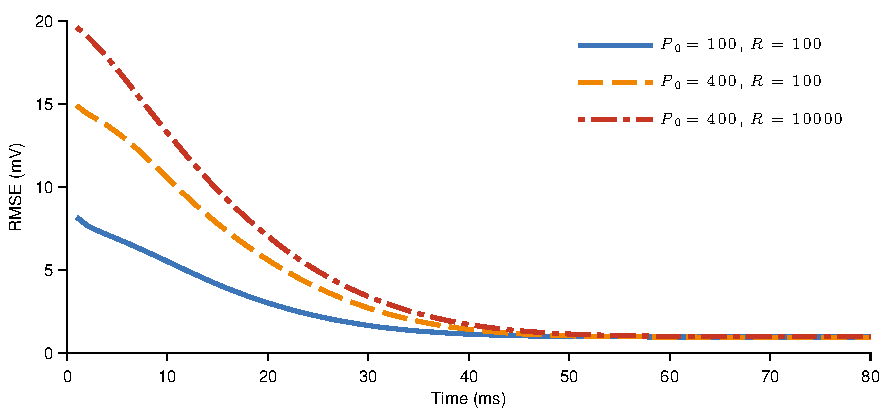
\includegraphics{./figures/pdf/DynamicCRB}
  \end{center}
  \caption{The evolution of the BCRB for of the first state of model A. The ... }
  \label{fig:DynamicCRB}
\end{figure}


\subsection{Across models - model feasibility}

We consider the feasibility of the three models described in Section~\ref{sec:background}. Models A and B contain 6 unknown states and model C has 10 unknown states. An important question to ask as the models become increasingly complex is: how well can we estimate the states from the available measurements? To investigate this, we compute the BCRB for each model in an operating mode analogous to alpha rhythms. The specific parameters are listed in Appendix~\ref{sec:parameter_table}.

\begin{figure}[ht]
  \begin{center}
    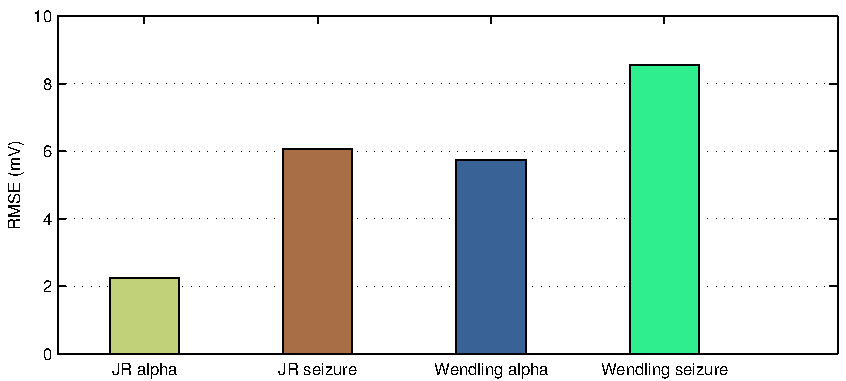
\includegraphics{./figures/pdf/AlphaSeizureBar}
  \end{center}
  \caption{The BCRB for two models in alpha and seizure states}
  \label{fig:AlphaSeizure}
\end{figure}



\subsection{Within model - seizure, alpha}

It has been well demonstrated that models of type B and C can generate vastly different oscillations for different parameters \cite{sdf}. Bifurcation theory provides a theoretical tool to analyze this feature and has been reported in several places \cite{sdf}. Good qualitative agreement between EEG data and the models has been observed and consequently different parameters sets have been assigned to different types of brain activity such as alpha rhythms or epileptic seizures \cite{sfd}.

Here, we investigate ones ability to estimate the states of a model for different types of activity. We calculate the BCRB for model B for two parameter sets representing alpha rhythms and epileptic seizures.

Fig.~\ref{fig:AlphaSeizure} illustrates that the states underlying seizure type behavior is more difficult to estimate than background alpha rhythms. This is expected since the input noise driving the system is amplified by a larger synaptic gain parameter, $A$, for the seizure state, as listed in Table~\ref{tbl:Parameters}. This increases the overall uncertainty in the model, reduces the information obtained by the measurements and thus increases the bound.

\subsection{Benchmark algorithms}

EKF doesn't reach bound for any nonlinear model, thus better algorithms are required.

\begin{figure}[ht]
  \begin{center}
    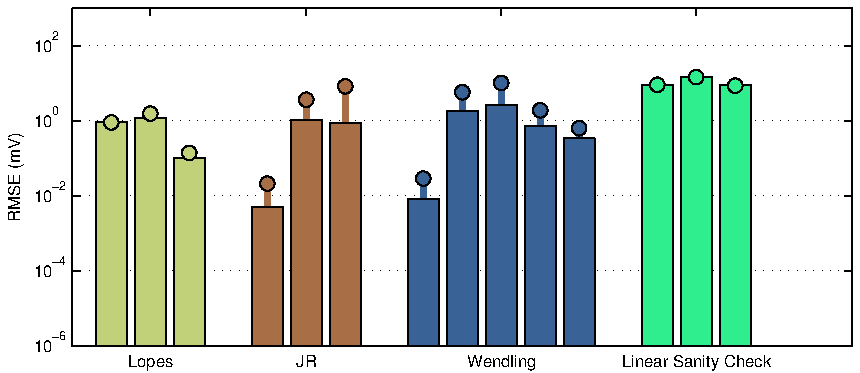
\includegraphics{./figures/pdf/CRBbar}
  \end{center}
  \caption{The mean squared error of the EKF against the BCRB for three models}
  \label{fig:CrbBar}
\end{figure}


\section{Discussion}
\brian{Brief Summary of Paper}
This paper has introduced a method for evaluating Bayesian estimation algorithms for fitting neural models to electrophysiological data. The results demonstrate that it is feasible to recover three neural models of varying complexity from data, by providing bounds on the possible estimation accuracy. Under the assumption that these models capture the essential dynamics of the phenomena observed in intracranial electroencephalography, the results imply that is possible to tailor computational models to an individual's brain dynamics. 

\brian{Feasibility of Models}
We have demonstrated how the methods described in this paper can be used to test the feasibility of recovering the states of computational models from data. In other words, the method can be used to test if a model is too complex to be recovered data, regardless of the estimation method. The Bayesian Cramer-Rao lower bound (BCRLB) essentially measures the amount of information regarding the states that is present in the measurement. If the measurement has no information regarding the states of the model, then the bound will be infinitely high. 

Mesoscopic neural models have evolved from a description of interaction of two very general populations, excitatory and inhibitory neurons, to interactions of specific populations that describe various networks. Cortical neural populations include pyramidal, spiny stellate, fast and slow inhibitory interneurons (ref). Deep brain populations include globus paladius, substansia niagara, sub-thalamic nuclei and more (ref). As models become more biologically realistic the BCRLB will be come more important for subject-specific modeling. Given that these models are simplified approximations of the brain, disturbances and modeling errors must be accounted for in the system equations. This naturally leads to Bayesian inference methods for subject-specific modeling to account for uncertainty. 

\brian{Is there a better observation to improve estimation? / experimental design}
In addition to evaluating estimation feasability and performance, the BCRLB can improve experimental design. For example, the bound can be used to select the nodes in a network that are important to measure in order to g. For example, 
sampling rate affects the CRLB, extensions to other applications e.g. experimental design
adaptive sensing

\brian{Calculating this provides an extra layer of intuition into the estimation process}
The evolution of the bound over time provides indication of convergence properties

derivatives higher -> more information

\brian{Stimulation / Excitation to maximize information}
Probing - maybe

\brian{Is there a better estimator?}
algorithm performance bench marking



\brian{Not model section}
Best case analysis which assumes the data comes from the model
we say nothing about how algorithms will work with uncertainty in the actual model -- thus can be considered a ``best case'' situation, where we know the true model exactly.
Model section still needs to be done by checking how the models can predict the behavior of the system. This need to be checked with test data set.

\brian{This method is the standard in radar and tracking and papers will not get published without it}
This is the first point of call for benchmarking estimation and tracking algorithms in the radar applications (refs). We argue that this should also be the case for neural state estimation and tracking. Neuroscience stands to benefit greatly from estimation and control techniques from engineering

\brian{Big picture}
Find the right level of model complexity and measurements to get to the truth.

\brian{What a subject specific model will provide the scientist and the neurologist}

contextualize work w.r.t. existing literature?


\section{Conclusion}

\appendix
\section{Derivation of Recursive Bayesian CRB}\label{sec:derivation_recursion}

The recursion in \cite{Bergman2001} is
\begin{subequations}
\begin{align}
	\mat P_{k|k-1} &= \bar{\mat F}_k\mat P_{k-1|k-1}\bar{\mat F}_k + \bar{\mat G}_k\mat Q_k \bar{\mat G}_k^{-1} \\
		\mat P_{k|k} &= \left(\mat P_{k|k-1}^{-1} + \bar{\mat R}_{k-1}^{-1}\right)^{-1}
\end{align}
\end{subequations}
where
\begin{align}
	\bar{\mat F}_k &= \mathbb E \left[ \nabla_{\vec x_k}^\top \tilde{\vec f_k}(\vec x_k,\vec v_k)\right] \\
	\bar{\mat R}_k^{-1} &= -\mathbb E\left[ \nabla_{\vec x_k}\nabla_{\vec x_k}^\top \log p(\vec y_k|\vec x_k) \right] \\
	\bar{\mat G}_k &= \mathbb E \left[ \nabla_{\vec v_k}^\top \tilde{\vec f_k}(\vec x_k,\vec v_k)\right] \\
	\mat Q_k^{-1} &= -\mathbb E \left[ \nabla_{\vec v_k}\nabla_{\vec v_k}^\top \log p(\vec v_k) \right]
\end{align}
and $\mat P_0^{-1}$ is the inverse of the prior covariance. The model in \eqref{eqn:model_general} is represented by $\tilde{\vec f}(\vec x_k,\vec v_k) = \vec f(\vec x_k) + \vec v_k$. This simplifies the derivatives to
\begin{align}
	\nabla_{\vec x_k}^\top \tilde{\vec f_k}(\vec x_k,\vec v_k) &= \mat F_k(\vec x_k) \\
	\nabla_{\vec v_k}^\top \tilde{\vec f_k}(\vec x_k,\vec v_k) &= \mat I_{d\times d} \\
	\nabla_{\vec x_k}\nabla_{\vec x_k}^\top \log p(\vec y_k|\vec x_k) &= -\mat H^\top\mat R^{-1} \mat H 
\end{align}
and the corresponding matrices to	
\begin{align}
	\bar{\mat F}_k &= \mathbb E\left[ \mat F_k(\vec x_k)\right] \label{eqn:pcrb_term_F}\\
	\bar{\mat R}_k^{-1} &= \mat H^\top\mat R^{-1} \mat H \\
	\bar{\mat G}_k &= \mat I_{d\times d} 
\end{align}
Therefore the final recursion is
\begin{align}
	\mat J_{k|k} = \left( \mat Q + \bar{\mat F}_{k-1} \mat J_{k-1}^{-1} \bar{\mat F}_{k-1}^\top\right)^{-1} + \mat H_k^\top \mat R^{-1} \mat H_k
\end{align}

\section{List of notation and parameters}
\label{sec:parameter_table}

Table here
\begin{table}
	
	\caption{\label{tbl:Parameters}Parameters used to generate different states}
\end{table}

\brian{\section*{Dean's Notes}
\subsection*{Definition of Sigmoid}
The error function version of the sigmoid is 
\begin{align}
	g(x) &= \frac{1}{2}\left(\mathrm{erf}\left(\frac{x-v_{0}}{\sqrt{2}\varsigma}\right) + 1\right).
\end{align}
This sigmoid is the cdf of a Gaussian, where $v_0$ is the mean and $\varsigma$ is the variance.
\subsection*{Transformation of GRV By erf}
Let
\begin{align}
	x\sim\mathcal{N}\left(\mu,\sigma^2\right)
\end{align}
and
\begin{align}
	y =& g(x) \\
	=& \frac{1}{2}\left(\mathrm{erf}\left(\frac{x-v_0}{\sqrt{2}\varsigma}\right) + 1\right).
\end{align}
Define some quantities to get transformed distribution:
\begin{align}
	x =& g^{-1}(y) \\
	  =& v_0 + \sqrt{2}\varsigma\mathrm{erf}^{-1}\left(2y-1\right) \\
	\frac{\mathrm{d}x}{\mathrm{d}y} =& \sqrt{2\pi}\varsigma\exp \left( \left[\mathrm{erf}^{-1}\left(2y-1\right)\right]^2\right)
\end{align}
The pdf of $y$ is
\begin{align}
	f_Y(y) =& \left|\frac{\mathrm{d}x}{\mathrm{d}y}\right|f_X(g^{-1}(y)) \\
	=& \frac{\varsigma}{\sigma}\exp\left(\left[\mathrm{erf}^{-1}\left(2y-1\right)\right]^2\right)\exp\left(-\frac{\left(v_0 + \sqrt{2}\varsigma\mathrm{erf}^{-1}\left(2y-1\right) - \mu\right)^2}{2\sigma^2}\right)
\end{align}
for $0<y<1$. Now let
\begin{align}
	z = \mathrm{erf}^{-1}\left(2y-1\right)
\end{align}
giving
\begin{align}
	f_Y(y)=& \frac{\varsigma}{\sigma}\exp\left(z^2\right)\exp\left(-\frac{\left(v_0 + \sqrt{2}\varsigma z - \mu\right)^2}{2\sigma^2}\right) \\
	=& \frac{\varsigma}{\sigma}\exp\left(-\frac{2\sigma^2 z^2 - \left(v_0 + \sqrt{2}\varsigma z - \mu\right)^2}{2\sigma^2}\right)
\end{align}
Get the numerator of the exponent in quadratic form
\begin{align}
	\mathrm{num} =& 2\left(\varsigma^2 - \sigma^2\right)z^2 + 2\sqrt{2}\varsigma\left(v_0-\mu\right)z + \mu^2 + v_0^2 - 2\mu v_0 \\
	=& az^2 + bz + c \\
	=& a\left(z-h\right)^2 + k
\end{align}
where
\begin{align}
	a =& 2\left(\varsigma^2 - \sigma^2\right) \nonumber \\
	b =& 2\sqrt{2}\varsigma\left(v_0-\mu\right) \nonumber \\
	c =& \mu^2 + v_0^2 - 2\mu v_0 \nonumber \\
	k =& c - \frac{b^2}{4a}\nonumber \\
	h =& - \frac{b}{2a}\nonumber
\end{align}
This gives
\begin{align}
	f_Y(y)=& \frac{\varsigma}{\sigma}\exp\left(\frac{k}{2\sigma^2}\right)\exp\left(-\frac{ (z - h)^2}{\frac{2\sigma^2}{a}}\right)
\end{align}
So we have a Gaussian like structure that may be exploited if we linearize $z$ (via first-order Maclaurin series expansion) such that
\begin{align}
	z =& \mathrm{erf}^{-1}\left(2y-1\right) \\
	\approx& \frac{\sqrt{\pi}}{2}\left(2y-1\right)
\end{align}
This may give and interesting alternative for Gaussian approximation filter??
\subsection*{Mode Derivation}
The Gaussian transformed by the error function sigmoid has the pdf
\begin{align}
	f_X(x)=& a\exp\left(-\frac{ \left(\mathrm{erf}^{-1}\left(2x-1\right) - b\right)^2}{c}\right)
\end{align}
Now let's find the mode. To simplify, first we take $\ln$ of $f_X(x)$ (since this will not shift the max) giving
\begin{align}
	\ln f_X(x)=& \ln a - \frac{ (\mathrm{erf}^{-1}\left(2x-1\right) - b)^2}{c}
\end{align}
Now find max by taking derivative and setting to zero. To do this we define
\begin{align}
	v =& 2x-1 \nonumber \\
	w =& \mathrm{erf}^{-1}(v) \nonumber \\
	y =& w-b \nonumber \\
	z =& y^2/c \nonumber
\end{align}
\begin{align}
	\frac{\mathrm{d}}{\mathrm{d}x} \ln f_X(x) =& 0
\end{align}
where
\begin{align}
	\frac{\mathrm{d}z}{\mathrm{d}y} \frac{\mathrm{d}y}{\mathrm{d}w} \frac{\mathrm{d}w}{\mathrm{d}v} \frac{\mathrm{d}v}{\mathrm{d}x} =& \frac{2y}{c} \times 1 \times \frac{\sqrt{\pi}}{2}\exp\left[\left(\mathrm{erf}^{-1}(v)\right)^2\right] \times 2 \\
	=& 0.
\end{align}
This is true where $y=0$. This implies the mode occurs at
\begin{align}
	\mathrm{erf}^{-1}(2x-1) = b.
\end{align}
From above
\begin{align}
	b = \frac{\sqrt{2}\varsigma\left(\mu-v_0\right)}{2\left(\varsigma^2-\sigma^2\right)}.
\end{align}
Therefore the mode is
\begin{align}
	\mathrm{mode}\left(f_X(x)\right) = \frac{1}{2}\left(\mathrm{erf}\left(\frac{\sqrt{2}\varsigma\left(\mu-v_0\right)}{2\left(\varsigma^2 - \sigma^2\right)}\right)+1\right)
\end{align}
This is correct and can be checked by code below.
}
\small
\bibliographystyle{ieeetr}
\bibliography{References}




\end{document}
